\chapter{慣性モーメント}

これまでは質点単体や, 複数の質点(質点系)について, 運動を考えてきた。
この章では, さらに進んで, 大きさと形を持つ物体の運動を考えよう。

\section{剛体というモデル}

第1章で述べたように, 大きさと形をもつ物体は, 質点の集まり
としてモデル化できる。ただし, 物体自体の変形(大きさや形が
変わること)まで考えると話が複雑になるので, ここでは, 
\begin{itemize}
\item 物体は質点の集まりで構成される。
\item 物体は大きさと形を持つ。
\item 物体は変形しない(ひとつの物体を構成する質点どうしの距離は変わらない)。
\end{itemize}
というようなモデルを考える。このような物体のモデルを
\underline{剛体}\index{ごうたい@剛体}(rigid body)という。

我々の身の回りの物体の多くは, 剛体とみなせる。カーリングストーンや, 
ボールなどは, これまでは質点とみなしてきたが, その大きさや形が
関与する運動(ボールの回転や, それによる軌道の変化等)
を考えるときは剛体として扱わねばならない。例えば地球は, 太陽
との位置関係を議論するときは質点でよいが, 地球の自転の様子を議論
するときは剛体とみなさねばならない。

ただし, 剛体も, 質点ほどではないが, 一種の単純化・抽象化されたモデルであり, 
問題設定によってはそれは不適切なこともある。例えば地球に起きる地震を考えるときは, 
地球を剛体とみなしてはダメであり, わずかながらも変形する弾性体として扱わねば
ならない\footnote{さらに言えば, 起きた振動(地震)が減衰して収まることを
表現するためには弾性体ではダメで, 摩擦も考慮した「粘弾性体」という物体
としてモデル化しなければならない。また, 物体が変形して元に戻らないことを表現するには, 
塑性というものも考えねばならず, 粘性や弾性も一緒に考慮するには「粘弾塑性体」
として考えねばならない。また, 水や空気のように流れる性質を持った物体は, 
「流体」として考えねばならない。このように, 扱う物体の性質や運動のスケール, 
本質的に関与する現象などによって, 物体をどのようにモデル化すべきかは様々だ。
複雑なモデルであればあるほどいいというわけではない。一般に, 様々な性質
を取り入れれば取り入れるほど, その問題を解くことは難しくなる。
従って, 本質を失わない範囲で, 扱う物体をできるだけ単純なモデルで
考える必要がある。}。\mv

さて, ここでは理由は詳述しないが, 剛体の運動は, 2つの要素にわけて考えることが
できる。ひとつはその「重心」の運動であり, もうひとつはその重心のまわりの
回転運動である(図\ref{fig:rigid_motion})。

\begin{figure}[h]
    \centering
    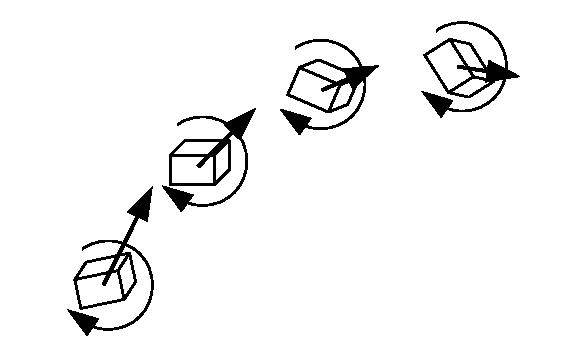
\includegraphics[width=5.0cm]{rigid_motion.eps}
    \caption{空中に放り投げられたレンガ。このような剛体の運動は, 重心の運動と, 重心まわりの回転で表現される。}\label{fig:rigid_motion}
\end{figure}
\hv

\section{剛体の回転運動}

ここでは剛体の回転運動について考えよう。

まず, 最も単純な場合として, 前章の問\ref{q:2points_rotation}で見たような, 
2つの質点がペアになって等速円運動(回転)することを考えよう(図\ref{fig:angular_mom_2balls}):
\begin{figure}[h]
    \centering
    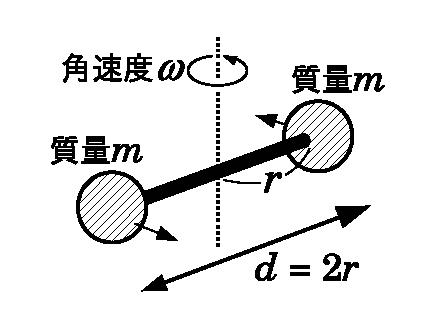
\includegraphics[width=4.0cm]{angular_mom_2balls.eps}
    \caption{棒でつながれた2つの質点からなる剛体の等速円運動。}\label{fig:angular_mom_2balls}
\end{figure}

2つの質点どうしの距離$d$が変わらないとき, この2つの質点からなる質点系は, 
剛体である。さて, このとき, 各質点の運動の速さ(速度の大きさ)$v$は, \eref{eq:circle_motion_v_romega}より
\begin{eqnarray}
v=r\omega
\end{eqnarray}
となる。従って, 各質点の運動エネルギーは, \eref{eq:kineticEnergy}より
\begin{eqnarray}
\frac{1}{2}mv^2=\frac{1}{2}m(r\omega)^2=\frac{1}{2}mr^2\omega^2\label{eq:rot_kineticE}
\end{eqnarray}
となる。従って, この剛体の運動エネルギー(つまり2つの質点の運動エネルギーの和)$T$は, 
\begin{eqnarray}
T=mr^2\omega^2\label{eq:rot_kineticE2}
\end{eqnarray}
となる。\eref{eq:rot_kineticE}のように, 各質点の(回転運動の)運動エネルギーが角速度の2乗に
比例するから, \eref{eq:rot_kineticE2}のように, 全質点の運動エネルギーの和も角速度の2乗に比例する。
同様に考えれば, 3個以上の質点が, ある固定点のまわりを同じ角速度で
等速円運動をしている場合についても, その回転による運動エネルギーは角速度の
2乗に比例すると類推できるだろう。\hv


\section{慣性モーメント}

そこで, 一般的に, 剛体が, ある軸のまわりに角速度$\omega$で回転
することを考えよう。剛体を, $n$個の微小な部分に分割し, それぞれを質量$m_1^{\,}, m_2^{\,}, ..., m_n^{\,}$
の質点とみなす。回転軸からそれぞれの質点への距離を$r_1^{\,}, r_2^{\,}, ..., r_n^{\,}$とする。
$k$番めの質点の速さ(速度の大きさ)は$r_k\omega$だから, 
$k$番目の質点の運動エネルギー$T_k^{\,}$は次式のようになる: 
\begin{eqnarray}
T_k=\frac{1}{2}m_k^{\,}r_k^2\omega^2
\end{eqnarray}
全体の回転の運動エネルギー$T$は, これらの全ての和であり, 
\begin{eqnarray}
T&=&T_1^{\,}+T_2^{\,}+\cdots+T_n^{\,}\nonumber\\
 &=&\frac{1}{2}m_1^{\,}r_1^2\omega^2+\frac{1}{2}m_2^{\,}r_2^2\omega^2+\cdots+\frac{1}{2}m_n^{\,}r_n^2\omega^2\nonumber\\
 &=&\frac{1}{2}(m_1^{\,}r_1^2+m_2^{\,}r_2^2+\cdots+m_n^{\,}r_n^2)\omega^2\nonumber\\
 &=&\frac{1}{2}\Bigl(\sum_{k=1}^{n}m_k^{\,}r_k^2\Bigr)\omega^2\label{eq:mominert00}
\end{eqnarray}
となる。\eref{eq:mominert00}の()内を抜き出して以下のように定義する:

\begin{itembox}{慣性モーメントの定義}
質量がそれぞれ$m_1, m_2, \cdots, m_n$であるような$n$個の
質点について,
\begin{eqnarray}
I=\sum_{k=1}^{n}m_k^{\,}r_k^2\label{eq:mominert_def}
\end{eqnarray}
で定義される物理量$I$を, \underline{慣性モーメント}\index{かんせいもーめんと@慣性モーメント}
(moment of inertia)もしくは\underline{慣性能率}\index{かんせいのうりつ@慣性能率}と呼ぶ。
ただし, $r_1, r_2, \cdots, r_n$は回転軸から各質点までの距離である。 
\end{itembox}

すると, 式(\ref{eq:mominert00})は以下のように書ける:
\begin{eqnarray}
T=\frac{1}{2}I\omega^2\label{eq:mominert}
\end{eqnarray}

%
\begin{q}\label{q:mominert_def} 
\begin{enumerate}
\item 慣性モーメントの定義を述べよ。
\item 慣性モーメントのSI単位は?
\end{enumerate}
\end{q}

%
\begin{q}\label{q:mominert_2points_rotation}
問\ref{q:2points_rotation}では, 慣性モーメントは$2mr^2$であることを示せ。
\end{q}
\mv

\eref{eq:mominert}を, 質点の運動エネルギー$T$の式(\eref{eq:kineticEnergy}で学んだ):
\begin{eqnarray}
T=\frac{1}{2}mv^2\quad\quad\text{($m$は質量, $v$は速度)}\label{eq:kineticEnergy9}
\end{eqnarray}
と比べてみよう。形式的によく似ている。実際, 形式的には, \eref{eq:kineticEnergy9}における速度$v$
と質量$m$は, \eref{eq:mominert}における角速度$\omega$と慣性モーメント$I$に対応する。
つまり, 形式的に言えば, 慣性モーメントとは「回転運動における質量みたいなもの」
である\footnote{注意: 同じ物体についても, 回転軸の位置や向きが違えば慣性モーメントも違う。ここでは深入り
しないが, 一般的に, 物体の慣性モーメントを任意の回転軸に関して完全に表現するには, 
行列(テンソル)を使う必要がある。何のことかよくわからぬ, という人は, とりあえず「ふーん...」
と思っておいてください。}。質量が物体の「動きにくさ」を表すとしたら, 慣性モーメントは
物体の「回りにくさ」を表す, と言ってもよかろう\footnote{もちろん, 既に動いている
物体については, むしろ質量は「止まりにくさ」であり, 慣性モーメントは「回転の止まりにくさ」
である。}。\mv

%
\begin{q}\label{q:mominert_3points}
半径$r$の円周上に, 質量$m$の質点が3個, 等間隔に並んで互いに固定されている(図\ref{fig:disk1})。このとき, 
円の中心を貫く垂線を軸とする回転の慣性モーメント$I$は?
\begin{figure}[h]
    \centering
    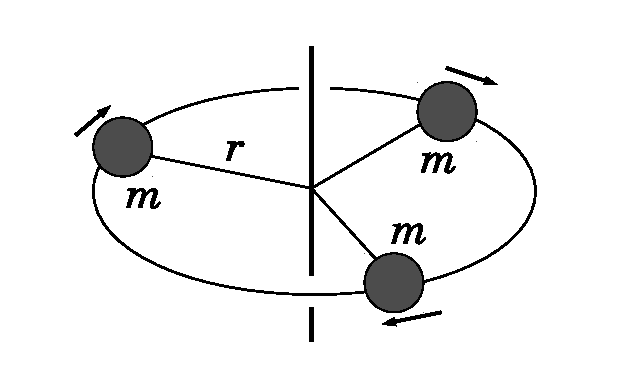
\includegraphics[width=3.5cm]{disk1.eps}
    \caption{3個の質点の回転}\label{fig:disk1}
\end{figure}
\end{q}

%
\begin{q}\label{q:mominert_npoints}
半径$r$の円周上に, 質量$m$の質点が$n$個, 等間隔に並んで互いに固定されている(図\ref{fig:disk2})。このとき, 
円の中心を貫く垂線を軸とする回転の慣性モーメント$I$は?
\begin{figure}[h]
    \centering
    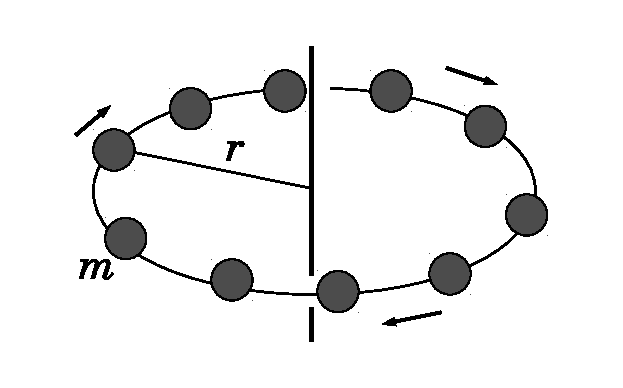
\includegraphics[width=3.5cm]{disk2.eps}
    \caption{$n$個の質点の回転}\label{fig:disk2}
\end{figure}
\end{q}
\vspace{0.2cm}

%
\begin{q}\label{q:mominert_ring}
前問で, 質量の合計, すなわち$nm$を$M$としよう。$M$を一定として$m$を小さくしながら$n$を無数に増やせば, これは質量$M$の円環に
なるだろう。そのように考えて, 半径$r$の円環(太さは無視できるほど小さいとする)の慣性モーメントは
\begin{eqnarray}
I=Mr^2\label{eq:mominert_ring}
\end{eqnarray}
となることを示せ(図\ref{fig:disk3})。
\begin{figure}[h]
    \centering
    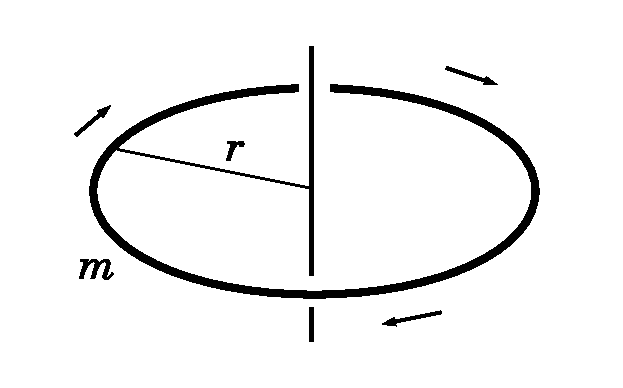
\includegraphics[width=3.5cm]{disk3.eps}
    \caption{円環の回転}\label{fig:disk3}
\end{figure}
\end{q}

%
\begin{q}\label{q:mominert_ringplate}
密度$\rho$, 厚さ$b$の鉄板でできた, 半径$r$, 幅$\Delta r$の円環盤について, 中心を貫く垂線を軸とする
回転の慣性モーメント$\Delta I$は, 
\begin{eqnarray}
\Delta I=2\pi\,\rho\,b\,r^3 \Delta r\label{eq:mominert_ringplate}
\end{eqnarray}
であることを示せ(図\ref{fig:disk4})。ただし$\Delta r$は$r$に較べて十分に小さい
ものとする。ヒント:$\Delta r$が十分に小さいから
円環盤は円環とみなせる。また, 円環盤の質量は, $2\pi r \rho b\Delta r$である。
\begin{figure}[h]
    \centering
    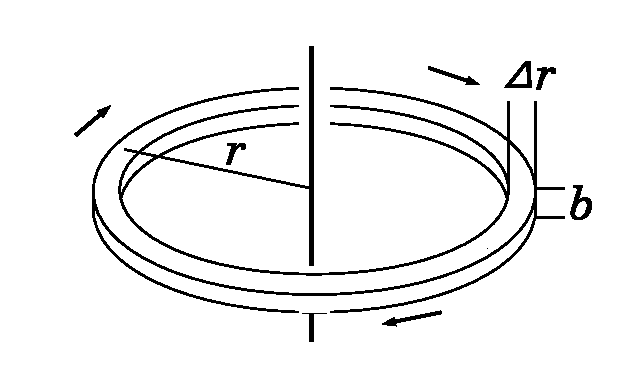
\includegraphics[width=3.5cm]{disk4.eps}
    \caption{円環盤の回転}\label{fig:disk4}
\end{figure}
\end{q}

%
\begin{q}\label{q:mominert_plate}
密度$\rho$, 厚さ$b$の鉄板でできた, 半径$r$の円盤について(図\ref{fig:disk5}), 
中心を貫く垂線を軸とする回転の慣性モーメント$I$は, 
\begin{eqnarray}
I=\frac{\pi\,\rho\,b\,r^4}{2}\label{eq:mominert_disk}
\end{eqnarray}
となることを示せ。ヒント:円盤は円環盤のあつまりとみなして, 前問の結果を様々な$r$について
適用して足しあわせる。$\Delta r$を十分小さくとれば, 足し合わせは積分になる。

また, この円盤の質量を$M$とすると, 
\begin{eqnarray}
I=\frac{Mr^2}{2}\label{eq:mominert_disc_horizon}
\end{eqnarray}
となることを示せ。これは, 同じ質量と半径を持つ円環の何倍か?
\begin{figure}[h]
    \centering
    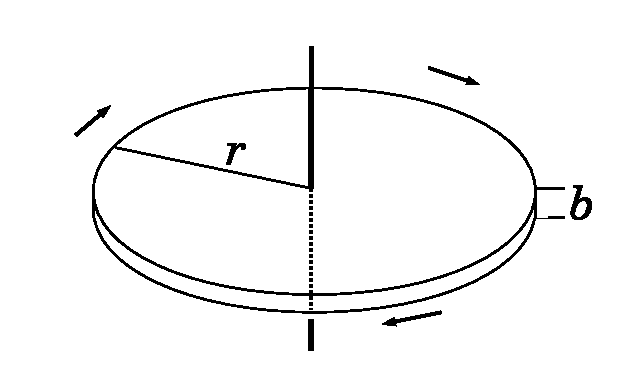
\includegraphics[width=3.5cm]{disk5.eps}
    \caption{円盤の回転}\label{fig:disk5}
\end{figure}
\end{q}

上の慣性モーメントの計算法をもう少し一般化しよう。任意の形状の連続的な剛体Vについて, 
それがひとつの軸の回りに回転することを考える。回転軸を$z$軸とし, それに直交するよう
に$x$軸と$y$軸を設定しよう。剛体Vを$x$軸, $y$軸, $z$軸に沿ってメッシュ状に分割し, 
横$\Delta x_i$, 縦$\Delta y_j$, 高さ$\Delta z_k$の小さな直方体(その中心の座標を
$(x_i, y_j, z_k)$とする。$i, j, k$は整数)のあつまりとみなす。
個々の部分の体積は$\Delta x_i \Delta y_j \Delta z_k$となり, その質量は$\rho \Delta x_i \Delta y_j \Delta z_k$
となる($\rho$は密度)。

\begin{figure}[h]
    \centering
    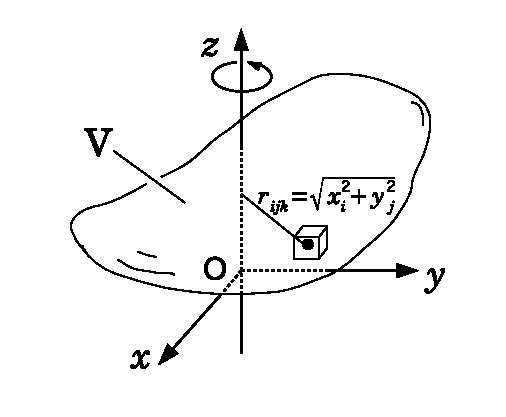
\includegraphics[width=5cm]{angular_mom_rigid.eps}
    \caption{連続的な剛体の回転}\label{fig:angular_mom_rigid}
\end{figure}

さて, 回転軸($z$軸)からの距離$r_{ijk}$の二乗は, 
\begin{eqnarray}
r_{ijk}^2=x_i^2+y_j^2
\end{eqnarray}
となる($z_k^2$は入らないことに注意せよ!)。すると慣性モーメント$I$は, \eref{eq:mominert_def}より, 
\begin{eqnarray}
I=\sum_{i}^{}\sum_{j}^{}\sum_{k}^{} \rho\, (x_i^2+y_j^2) \Delta x_i \Delta y_j \Delta z_k\label{eq:mominert_rigid_sigma}
\end{eqnarray}
となる。ここで$\Delta x_i, \Delta y_j, \Delta z_k$を限りなく小さくすると, 
それぞれの和は積分に置き換えられ, 次式のようになる:
\begin{itembox}{連続的な剛体の慣性モーメントの定義}
\begin{eqnarray}
I=\int_{}^{}\int_{}^{}\int_{\text{V}}^{}\,\, \rho\,(x^2+y^2)\,dx\,dy\,dz\label{eq:mominert_rigid_integ}
\end{eqnarray}
\end{itembox}
この積分は「体積分」であり(わからない人は数学の教科書を参照せよ), 積分区間は, 剛体Vの隅から隅までである。\mv

%
\begin{q}\label{q:mominert_r2}
上の\eref{eq:mominert_rigid_sigma}や\eref{eq:mominert_rigid_integ}において, 
カッコの中(つまり$r^2$)が$x^2+y^2+z^2$でないのはなぜか? ($z^2$を入れてはいけない
のはなぜか? )
\end{q}
\mv

\begin{q}\label{q:mominert_diameter}
問\ref{q:mominert_plate}で扱ったのと同じ円盤について, ある直径を軸とする回転の
慣性モーメント(図\ref{fig:disk6})が次式のようになることを示せ。
\begin{eqnarray}
I=\frac{Mr^2}{4}\label{eq:mominert_disc_diameter}
\end{eqnarray}
\begin{figure}[h]
    \centering
    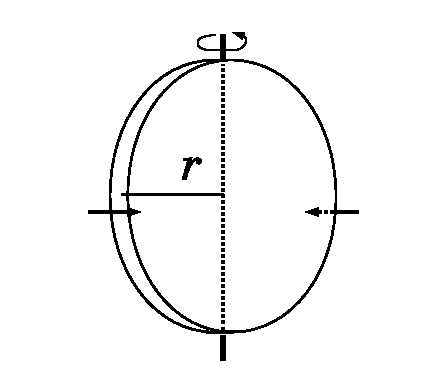
\includegraphics[width=3.5cm]{disk6.eps}
    \caption{円盤の回転。ただし縦回転。}\label{fig:disk6}
\end{figure}
\end{q}

\eref{eq:mominert_disc_horizon}と\eref{eq:mominert_disc_diameter}を比べれば
わかるように, 同じ物体であっても, 回転軸をどのように設定するかによって, 慣性モーメント
は異なる値をとる。ここでは詳述しないが, 互いに直交する3つの回転軸を適切に定めて
それらのまわりの慣性モーメントを求めれば, それをもとに, どんな方向の回転軸についても
慣性モーメントを自動的に計算することができる。数学的には, その「適切な3つの
回転軸」と「そのまわりの慣性モーメント」を求めることは, 行列(対称行列)の
固有ベクトルと固有値を求めることに対応する。興味のある人は, しっかりした力学の
教科書を参照してみよう。\mv

慣性モーメントは, 農業機械の設計などで重要だ。耕運機は, どのような形・
質量のロータリーを搭載するかで大きく性能が決まるが, そのロータリーを駆動するのに
どのくらいの出力のエンジンが必要か, などという判断は, 慣性モーメントを含む
力学的見地からの設計にかかっている。出力の大きなエンジンならどんな慣性モーメント
を持つロータリーも動かせるが, その反面, 重くなるので操作性が悪くなるし, 
燃費も悪くなる。

大きな慣性モーメントを持つ物体, 例えば大きな鉄の円盤などが回転すると, 大きな
運動エネルギーを持つ。これは, エネルギーの貯蔵装置として利用できる。例えば
太陽光や風力などの不安定なエネルギー源でも, エネルギーが得られるときには
大きな鉄円盤を回すことができる。いったんまわり始めた鉄円盤は, 角運動量保存則
でまわり続けるので, エネルギーが欲しいときに鉄円盤の回転で発電機を回して
エネルギーを取り出すことができる。このようなエネルギー貯蔵装置を
フライホイール\index{ふらいほいーる@フライホイール}と呼ぶ。\mv

%
\begin{q}\label{q:mominert_wheel_slope}
傾斜$\theta$, 高さ$h$の坂の上から, 半径$r$, 質量$M$, 慣性モーメント$I$の
丸い物体Xを転がそう(図\ref{fig:slope_wheel})。
坂と物体の間に摩擦は生じないものとする。重力加速度を$g$とする。
\begin{figure}[h]
    \centering
    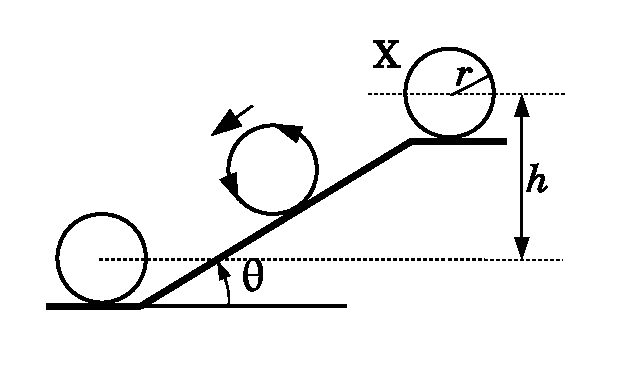
\includegraphics[width=6.0cm]{slope_wheel.eps}
    \caption{斜面を転がり下る丸い物体X。}\label{fig:slope_wheel}
\end{figure}\begin{enumerate}
\item Xのポテンシャルエネルギーを$U$とする。Xが坂の下にあるとき$U=0$とする。Xが坂の上にあるときの$U$は?
ただし, 一般的に, 一様な外力(重力など)による剛体(変形しない物体)のポテンシャルエネルギーは, 
質量が全て重心(この場合はXの中心)に集中すると仮想したときの質点のポテンシャルエネルギーに等しいことがわかっている。
\item Xは坂の上から初速度0で転がり出す。Xが転がり出したとき(速度は0)の力学的エネルギー$E_0$は?
\item Xが坂の下まで到達したとき, 重心(Xの中心)の速度は$v$, 回転の角速度は$\omega$であった。このとき, 
\begin{eqnarray}
v=r\omega
\end{eqnarray}
が成り立つことを示せ。ヒント:ごく短い時間間隔$\Delta t$の間($v$や$\omega$が一定とみなせるくらいに
短い時間間隔)に, Xは$r\omega\Delta t$だけ進む。
\vspace{0.1cm}
\item Xが坂の下まで到達したとき, Xの力学的エネルギー$E_1$は, 
\begin{eqnarray}
E_1=\frac{M\,v^2}{2}+\frac{I\omega^2}{2}
\end{eqnarray}
となることを示せ。ただし, 運動エネルギーは重心の運動エネルギー(全質量が重心に集中した仮想的な質点の
運動エネルギー)と重心まわりの回転の運動エネルギーの和であることがわかっている。
\item 力学的エネルギー保存則($E_0=E_1$)から, 以下の式を導け:
\begin{eqnarray}
Mgh=\frac{M\,v^2}{2}+\frac{I\omega^2}{2}
\end{eqnarray}
\item (3)で得た関係と前問から, 以下の式を導け:
\begin{eqnarray}
2gh=v^2\Bigl(1+\frac{I}{M\,r^2}\Bigr)\label{eq:mominert_wheel_slope3}
\end{eqnarray}
\item 前問から, 以下の式を導け:
\begin{eqnarray}
v=\sqrt{\frac{2g\,h}{1+I/(M\,r^2)}}\label{eq:mominert_wheel_slope_v}
\end{eqnarray}
\item 慣性モーメント$I$が0の場合, $v=\sqrt{2g\,h}$となることを示せ。これは質量$M$の質点が坂を
滑り降りるときの速度に等しい。
\item Xが, 質量$M$が縁に集中している円環の場合, $v=\sqrt{g\,h}$となることを示せ。
\item Xが, 質量$M$が一様に分布している円盤の場合, $v$はどうなるか?
\end{enumerate}
\end{q}
\mv

%
\begin{q}\label{q:mominert_ball_slope}
坂の上から, 同じ半径の2つの鉄球を転がす。鉄球Aは, 内部が空洞であり, 鉄球Bは, 内部までびっちり鉄が
詰まっている。どちらが速く転がるか? 理由も述べよ。
\end{q}
\hv


\section{分子の運動と慣性モーメント}

%2011.4.5 ヤマサキ 8章との整合をとった。(この辺の内容は少し自信がないので, 書いてあることが変じゃないかよく確かめてもらえるとありがたいです)
慣性モーメントは化学でも重要だ。多原子分子は, 温度に応じて, 並進と振動と
回転という3種類の運動をする\footnote{ただし常温では, 振動運動は熱にあまり関係しない。}。
この回転運動の性質を解析することで, 分子の様子を調べることができる。

例として, 質量$m$の原子2個からなる2原子分子を考える。原子間の距離を$d$とする。重心は
原子どうしの中間点にある。2つの原子を結ぶ直線に垂直で重心を通るひとつの直線を軸とする, 
回転運動を考える(図\ref{fig:angular_mom_H2})。重心から各原子までの距離を$r$とする。
当然, $d=2r$だ。
\begin{figure}[h]
    \centering
    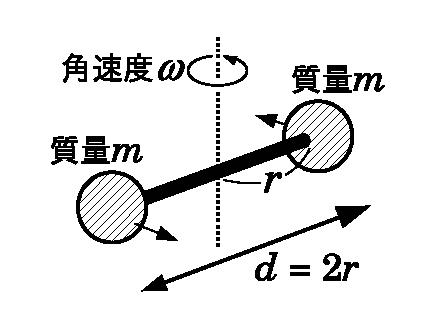
\includegraphics[width=4.5cm]{angular_mom_2balls.eps}
    \caption{2原子分子の回転。}\label{fig:angular_mom_H2}
\end{figure}

P.\pageref{def:temperature0}で学んだエネルギー等分配則によれば, 
一般に, 絶対温度$T$の
気体の1分子は, ひとつの自由度につき, $k_{\text{B}}T/2$という運動エネルギーを
平均的に持つ。今考えている回転運動も1つの自由度を持った運動といえるので, 
この回転に関する平均的な運動エネルギー$K$は, 
\begin{eqnarray}
K=\frac{1}{2}k_{\text{B}}T\label{eq:2atommolrot1}
\end{eqnarray}
である\footnote{これまで運動エネルギーは$T$で表すことが多かったが, この問題では
$T$は温度を表すので, それとの混乱を避けるために, 運動エネルギーを$K$と書いた。}。
一方, この原子の慣性モーメント$I$は, 問\ref{q:mominert_2points_rotation}より, 
$I=2mr^2$だ。従って, 次式が成り立つ:
\begin{eqnarray}
K=\frac{1}{2}I\omega^2=mr^2\omega^2\label{eq:2atommolrot2}
\end{eqnarray}

%
\begin{q}\label{q:mominert_molecule}
この2原子分子について, 
\begin{enumerate}
\item 次式を示せ:
\begin{eqnarray}
\omega=\frac{1}{r}\sqrt{\frac{k_{\text{B}}T}{2m}}\label{eq:2atommolrot3}
\end{eqnarray}
\item 窒素原子$^{14}$Nと$^{15}$Nの質量をそれぞれ$m_1$, $m_2$とする。これらを求めよ。
\item 窒素分子の原子間距離は, $d=0.11\text{ nm}$である。常温(300 K)における, 
$^{14}$N$_2$分子の回転の角速度$\omega_1$と, 
$^{15}$N$_2$分子の回転の角速度$\omega_1$を調べよ。両者にはどのくらいの差があるか?
\end{enumerate}

諸君は, 元素の同位体は化学的特性が同じなので, 化学的に分別することは難しい
と習っただろう。しかし, この問題でわかるように, 異なる同位体は, 同じ温度のもとでも
異なる回転速度を持つ。ちなみに, この問題で扱った方法は, ニュートン力学に基づくものであり, 古典的と言われる。
実際は, 分子の回転運動をこのように古典的に扱うことは適当ではなく, 量子力学を
使わねばならない。その違いを手短に言うと, 量子力学的な扱いでは, 
回転運動の角速度という概念は意味を持たない。そのかわりに, 
角運動量をもとに理論を組み立てる。その際, 古典的な意味での角運動量では考えられない
ようなことが起きる。しかし, このような古典的な扱いでも, いろんなことがわかるし, 
量子力学的な扱いをするときに考え方の出発点となる。
\hv

\section{剛体振り子}

2学期の「物理学実験」では, 振り子を利用して重力加速度を測る実験が行われる。そこでは, 
問\ref{q:furiko_energy}で学んだ, 糸に質点がつるされた振り子でなく, 剛体の振り子
\index{ふりこ@振り子}を使う。ここではその予習をしておこう。\mv

\begin{q}\label{q:mominert_pandulum}
質量$M$の剛体に穴が開けられ, その穴に軸を通して, その軸が定点Pに固定されている
(図\ref{fig:solid_pendulum})。剛体は軸のまわりに自由に回転することができる。
軸のまわりの回転の慣性モーメントを$I$とする。剛体の重心をGとする。PからGの距離
は$l$である。Gが最も下に来たときの位置をOとする。剛体を少し持ち上げて静かに手放すと, 
重心Gは鉛直平面内で振動運動をする。時刻$t$における重心の位置をG($t$)とし, 角OPGを$\theta(t)$と
しよう。空気抵抗は無視する。
\begin{figure}[h]
    \centering
    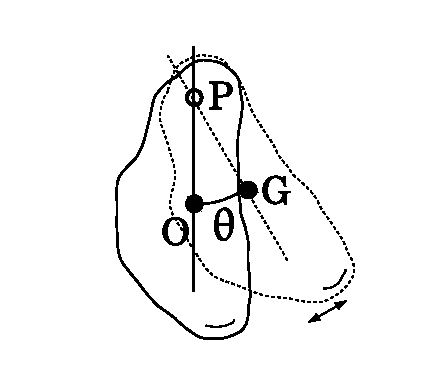
\includegraphics[width=6cm]{solid_pendulum.eps}
    \caption{剛体振り子。}\label{fig:solid_pendulum}
\end{figure}
\begin{enumerate}
\item 時刻$t$における剛体の運動エネルギー$T(t)$は次のようになることを示せ:
\begin{eqnarray}T(t)=\frac{1}{2}\,I\,\Bigl(\frac{d\theta}{dt}\Bigr)^2\end{eqnarray}
\item 時刻$t$におけるこの剛体のポテンシャルエネルギー$U(t)$は次のようになることを示せ。
\begin{eqnarray}U(t)=M\,g\,l\,(1-\cos \theta)\end{eqnarray}
ただし, Gが点Oにあるとき$U=0$と定める。
\item 力学的エネルギー保存則から, 次式(剛体振り子の運動をあらわす方程式)を得よ:
\begin{eqnarray}
I\frac{d^2\theta}{dt^2}=-M\,g\,l\sin\theta\label{q:mominert_pandulum5}
\end{eqnarray}
\item ここで「等価振り子の長さ」\index{とうかふりこのながさ@等価振り子の長さ}というものを, 
\begin{eqnarray}
\overline{l}=\frac{I}{M\,l}\label{q:mominert_pandulum6}
\end{eqnarray}
と定義し, $\overline{l}$を使って上の方程式を書き換えると, 質点の振り子の方程式(式(\ref{eq:furiko_equation}))と同じ形
\begin{eqnarray}
\frac{d^2\theta}{dt^2}=-\frac{g}{\overline{l}}\sin\theta\label{q:mominert_pandulum7}
\end{eqnarray}
となることを示せ。
\item 角$\theta$が十分に0に近い範囲で変化するならば, \eref{q:mominert_pandulum7}は次の
ように近似できることを示せ:
\begin{eqnarray}
\frac{d^2\theta}{dt^2}=-\frac{g}{\overline{l}}\theta\label{q:mominert_pandulum8}
\end{eqnarray}
\item 上の方程式について, $\theta=\theta_0 \cos \omega t$という式を仮定して代入し, 
振動の角速度$\omega$を求め, 振動の周期$T$が次式のようになることを示せ:
\begin{eqnarray}
T=2\pi\sqrt{\frac{\overline{l}}{g}}\label{q:mominert_pandulum9}
\end{eqnarray}
\item 次式を導け(これは「物理学実験」テキストのテーマ3の(2)式と同じ):
\begin{eqnarray}g=\Bigl(\frac{2\pi}{T}\Bigr)^2\overline{l}\end{eqnarray}

\end{enumerate}
\end{q}
\mv

慣性モーメント$I$は, 剛体の回転運動の運動エネルギーを\eref{eq:mominert}のように表すために
定義された。しかし, 慣性モーメントの効用は, もうひとつある: 理由は詳述しないが, 
剛体の角運動量の大きさ$L$は, 
\begin{eqnarray}
L=I\omega\label{eq:mominert_angmom}
\end{eqnarray}
と表すことができる\footnote{以下, 参考までに述べておく(今は理解できなくてもよい)。
\eref{eq:mominert_angmom}は, 実はベクトルの方程式に拡張できるのだ。
すなわち, 角運動量は本来はベクトルなので${\bf L}$と表そう。角速度は, 回転軸の方向を向いている
ベクトル量とみなすことができて, それを$\pmb{\omega}$とおこう。慣性モーメントは, 先述のように, 
実は行列で表現できる。それを改めて$I$とおこう。すると, \eref{eq:mominert_angmom}は, 
\begin{eqnarray}
{\bf L}=I\pmb{\omega}\label{eq:mominert_angmom_vect}
\end{eqnarray}
\mv
となるのだ。}。\mv

%
\begin{q}\label{q:mominert_earthquake}
2011年3月に発生した, 東北太平洋沖地震の後, 地球の
自転周期が1.8マイクロ秒だけ短くなった(自転が早くなった)
ことが観測された。この現象を慣性モーメントの考え方を使って定性的に
説明せよ。
\end{q}

\begin{faq}{\small\textgt{私はクラシック・バレエをやっています。バレエでも, フィギュアスケートで言う
スピンと同じことを地表で行い(踊り)ますが, 腕をうまくタイミング良く体の中心に引き寄せると
速く且つ安定して回れます。} ... 
これは問\ref{q:mominert_earthquake}と同じ原理です。回転現象は本当に不思議ですね。}\end{faq}

\begin{faq}{\small\textgt{物体の運動をここまで数式で予測できるなんて凄い
ですが, 実際に自分では思いつける気がしません。やはり私に物理は無理って感じです}
 ... 大丈夫。ここまで物理学が発展するのに何千年間もかかったのです。
20歳くらいの若者がすぐに理解したり思いつけるようなものではありません。
先人の業績をもとに, 真理を謙虚に学べばそれでよいのです。
}\end{faq}
\hv

\section{解答}
\noindent{\textbf{答}}\ref{q:mominert_def} 
(1) 略。(2)\eref{eq:mominert_def}より, $I$の単位は$m_kr_k^2$の単位なので, kg~m$^2$
\mv

\noindent{\textbf{答}}\ref{q:mominert_2points_rotation}
\eref{eq:mominert_def}で$n=2$, $r_1=r_2=r$, $m_1=m_2=m$とすればよい。
$I=m\,r^2+m^{\,}r^2=2m^{\,}r^2$

\noindent{\textbf{答}}\ref{q:mominert_3points}
\eref{eq:mominert_def}で$n=3$, $r_k=r$, $m_k=m$とすればよい。
$I=3m\,r^2$

\noindent{\textbf{答}}\ref{q:mominert_npoints}
\eref{eq:mominert_def}で, $r_k=r$, $m_k=m$とすればよい。
$I=nm\,r^2$

\noindent{\textbf{答}}\ref{q:mominert_ring}
前問で$nm=M$とすれば与式を得る。\mv

\noindent{\textbf{答}}\ref{q:mominert_ringplate}
円環盤も円環の一種だ。この円環盤をどこか1箇所で切ってまっすぐに
伸ばしたら, 断面積は$b\Delta r$, 長さは$2\pi r$の鉄棒になる。その体積は
$2\pi br \Delta r$。密度が$\rho$なので, 質量は$2\pi\rho br \Delta r$。
これを$M$として\eref{eq:mominert_ring}に代入すると与式を得る(ただしここでは
慣性モーメントを$I$でなく$\Delta I$と書いていることに注意)。\mv

\noindent{\textbf{答}}\ref{q:mominert_plate}
円盤を$\Delta r$の幅の$n$個の円環盤に分割し, \eref{eq:mominert_ringplate}
で与えられる各円環盤の慣性モーメントを足し合わせると, 円盤の慣性モーメント$I$になるはず
だ。すなわち, 次式のように書ける:
\begin{eqnarray}
I=\sum_{k=1}^{n}2\pi\,\rho\,b\,r_k^3 \Delta r
\end{eqnarray}
ここで$r_k$は$k$番目の円環盤の半径である。
分割をどんどん細かくして$\Delta r$を十分に0に近づけ, 円環の数を
どんどん増やすならば, この式は次式のようになる: 
\begin{eqnarray}
I=\int_{0}^{R}2\pi\,\rho\,b\,r^3\,dr
\end{eqnarray}
ここで$R$は円盤の半径である。この積分を実行すると, 
$I=\pi\,\rho\,b\,R^4/2$。
ここで改めて$R$を$r$に置き換えると, \eref{eq:mominert_disk}を得る。
ところで, この円盤の質量$M$は, $M=\pi\,\rho\,b\,r^2$
なので, \eref{eq:mominert_disk}より$I=M\,r^2/2$
となり, \eref{eq:mominert_disc_horizon}を得る。これは同質量の円環の慣性モーメント, 
つまり\eref{eq:mominert_ring}の半分である。\mv

\noindent{\textbf{答}}\ref{q:mominert_r2}
慣性モーメントの本来の定義, つまり\eref{eq:mominert_def}では, 
$r_k$は原点からの距離ではなく, 回転軸からの距離だった。連続的な
剛体に関する慣性モーメントも事情は同じだ。従って, 剛体の
各部分について, $r$として原点からの距離つまり$\sqrt{x^2+y^2+z^2}$
ではなく, 回転軸($z$軸)からの距離つまり$\sqrt{x^2+y^2}$を
考えねばならない。\mv

\noindent{\textbf{答}}\ref{q:mominert_diameter}
回転軸を$z$軸, それに直交して円盤の直径方向に$x$軸, 厚さ方向に
$y$軸をとる。円盤の中心を原点とする。円盤の厚さを$b$とする。
密度を$\rho$とする。円盤上の点$(x, y, z)$と$z$軸との距離は$\sqrt{x^2+y^2}$だ。
慣性モーメント$I$は, \eref{eq:mominert_rigid_integ}より
\begin{eqnarray*}
I=\int_{-r}^{r}\int_{-b/2}^{b/2}\int_{-\sqrt{r^2-z^2}}^{\sqrt{r^2-z^2}}\rho(x^2+y^2)\,dx\,dy\,dz
\end{eqnarray*}
である。ここで円盤が十分に薄いとすれば, $x^2+y^2\fallingdotseq x^2$であり, その
近似のもとに, $y$について先に積分すれば, 
\begin{eqnarray}
I&=&b\int_{-r}^{r}\int_{-\sqrt{r^2-z^2}}^{\sqrt{r^2-z^2}}\rho x^2\,dx\,dz
\end{eqnarray}
となる。これを$x$について積分すれば, 
\begin{eqnarray*}
I=b\int_{-r}^{r}\Bigl[\rho\frac{x^3}{3}\Bigr]_{-\sqrt{r^2-z^2}}^{\sqrt{r^2-z^2}}\,dz
=\frac{2b\rho}{3}\int_{-r}^{r}(r^2-z^2)^{3/2}\,dz
\end{eqnarray*}
となる。この被積分関数は$z$に関する偶関数だから, 
\begin{eqnarray}
I=\frac{4b\rho}{3}\int_{0}^{r}(r^2-z^2)^{3/2}\,dz
\end{eqnarray}
となる。ここで$z=r\sin\theta$と置換すると(置換積分), 
$dz=r\cos\theta\,d\theta$であり, 積分区間は$0\leq\theta\leq\pi/2$であり, 
被積分関数は
$(r^2-z^2)^{3/2}=(r^2-r^2\sin^2\theta)^{3/2}
               =\{r^2(1-\sin^2\theta)\}^{3/2}
               =(r^2\cos^2\theta)^{3/2}=r^3\cos^3\theta$。
従って, $I=$
\begin{eqnarray*}
\frac{4b\rho}{3}\int_{0}^{\pi/2}r^3\cos^3\theta\,r\cos\theta\,d\theta
 =\frac{4br^4\rho}{3}\int_{0}^{\pi/2}\cos^4\theta\,d\theta
\end{eqnarray*}
ところで, オイラーの公式から, 
\begin{eqnarray}
\cos^4\theta&=&\Bigl(\frac{e^{i\theta}+e^{-i\theta}}{2}\Bigr)^4\nonumber\\
             &=&\frac{e^{4i\theta}+4e^{2i\theta}+6+4e^{-2i\theta}+e^{-4i\theta}}{16}\nonumber\\
             &=&\frac{e^{4i\theta}+e^{-4i\theta}}{16}+\frac{e^{2i\theta}+e^{-2i\theta}}{4}+\frac{3}{8}\nonumber\\
             &=&\frac{\cos 4\theta}{8}+\frac{\cos2\theta}{2}+\frac{3}{8}
\end{eqnarray}
従って, 
\begin{eqnarray}
I&=&\frac{4br^4\rho}{3}\int_{0}^{\pi/2}\Bigl(\frac{\cos 4\theta}{8}+\frac{\cos2\theta}{2}+\frac{3}{8}\Bigr)\,d\theta\nonumber\\
 &=&\frac{4br^4\rho}{3}\Bigl[\frac{\sin 4\theta}{32}+\frac{\sin2\theta}{4}+\frac{3\theta}{8}\Bigr]_0^{\pi/2}\nonumber\\
 &=&\frac{4br^4\rho}{3}\frac{3\pi}{16}=\frac{\pi br^4\rho}{4}=\frac{Mr^2}{4}
\end{eqnarray}
ここで, $M=\pi b r^2 \rho$を使った。\mv

\noindent{\textbf{答}}\ref{q:mominert_wheel_slope}
(1) $U=Mgh$。
(2) 速度が0なので, 運動エネルギーは0。従って力学的エネルギー$E_0$はポテンシャルエネルギー$U$
だけだ。(1)より, $E_0=Mgh$
(3) $r\omega\Delta t/\Delta t=r\omega$
(4) 重心の運動エネルギーは, 
$Mv^2/2$であり, 回転の運動エネルギーは
$I\omega^2/2$である。これらを足すと, 与式を得る。
(5) (1)と(4)より, 与式を得る。
(6) 前小問の式に(3)の結果を代入して$v$を消すと, 
\begin{eqnarray}
Mgh=\frac{M\,r^2\omega^2}{2}+\frac{I\omega^2}{2}
\end{eqnarray}
となる。両辺を2倍して$M$で割ると, 与式を得る。
(7) 略(\eref{eq:mominert_wheel_slope3}を$v=$の形に式変形すればよい)。
(8) 略(\eref{eq:mominert_wheel_slope_v}に$I=0$を代入するだけ)。
(9) \eref{eq:mominert_ring}を\eref{eq:mominert_wheel_slope_v}に代入して与式を得る。
(10) \eref{eq:mominert_disc_horizon}を\eref{eq:mominert_wheel_slope_v}に代入して, 
$v=\sqrt{4g\,h/3}$
\mv

\noindent{\textbf{答}}\ref{q:mominert_ball_slope}
\eref{eq:mominert_wheel_slope_v}より, 慣性モーメント$I$と質量$M$の比($I/M$)
が小さいほど転がる速さは大きい。$I/M$は, 質量が回転軸に近い部分に集中するほど小さい。
鉄球Aは内部が空洞なので, 質量は回転軸から遠い部分に分布するが, 鉄球Bは質量が回転軸に
近いところにも(鉄球Aに比べると)多く分布する。従って, $I/M$は鉄球Bの方が小さい。
従って, 鉄球Bの方が速く転がる。\mv


\noindent{\textbf{答}}\ref{q:mominert_molecule} 略。(3)は10$^{12}$/s〜10$^{13}$/s程度の量になる。
%\begin{enumerate}
%\item \eref{eq:2atommolrot1}と\eref{eq:2atommolrot2}がともに成り立つとし, 
%$\omega$について解けばよい。
%\item 酸素原子は原子量16である。つまり, 1モルが16~gである。従って, 酸素原子1個の質量は, 
%\begin{eqnarray*}
%m&=&\frac{16\times10^{-3}\text{ kg}}{6.0\times10^{23}}=2.7\times10^{-26}\text{ kg}
%\end{eqnarray*}
%\item \eref{eq:2atommolrot3}を使う。
%\begin{eqnarray*}
%r=\frac{d}{2}=\frac{0.12\times10^{-9}\text{ m}}{2}=6.0\times10^{-11}\text{ m}
%\end{eqnarray*}
%より. 
%\begin{eqnarray*}
%\omega=\frac{1}{6.0\times10^{-11}\text{ m}}\sqrt{\frac{1.38\times10^{-23}\text{ J K}^{-1}\times300\text{ K}}{2\times2.7\times10^{-26}\text{ kg}}}\\
%=4.6\times10^{12}\text{ s}^{-1}
%\end{eqnarray*}
%\end{enumerate}
\mv

\noindent{\textbf{答}}\ref{q:mominert_pandulum} 
(1) 剛体の振動運動は, ごく短い時間を切り出して考えれば, 軸を中心とする
回転運動の一部とみなすことができる。その角速度$\omega$は, 単位時間あたり
に変化する角なので, $\theta$を時刻$t$で微分したものに等しい。従って, 
$\omega=d\theta/dt$である。これを\eref{eq:mominert}に代入して, 与式を得る。
(2) 剛体の(重力による)ポテンシャルエネルギーは, 基準点からの重心の高さと全質量, そして
重力加速度をかけたものに等しい。題意より, 定点(軸の位置)Pから原点Oまでの距離は$l$である。
Pから重心Gまでの距離も$l$だが, 剛体が角$\theta$だけ傾いているときは, PとGの高さの
差は, $l\cos\theta$となる。従って, 原点Oと重心Gの高さの差は$l-l\cos\theta$となる。
従って, ポテンシャルエネルギーは与式のようになる。
(3) 力学的エネルギー保存則より, $T(t)+U(t)$は時刻によらぬ定数である。従って, 
$T(t)+U(t)$を$t$で微分したら恒等的に0になる。従って,
\begin{eqnarray*}
&&\frac{d}{dt}\{T(t)+U(t)\}\\
&&=\frac{d}{dt}\Bigl\{\frac{1}{2}\,I\,\Bigl(\frac{d\theta}{dt}\Bigr)^2+M\,g\,l\,(1-\cos \theta)\Bigr\}\\
&&=I\,\Bigl(\frac{d\theta}{dt}\Bigr)\Bigl(\frac{d^2\theta}{dt^2}\Bigr)+M\,g\,l\,\sin \theta\,\frac{d\theta}{dt}=0
\end{eqnarray*}
この式から与式を得る。
(4) 略(\eref{q:mominert_pandulum6}を使って\eref{q:mominert_pandulum5}から$I$を
消去すると\eref{q:mominert_pandulum7}を得る)。
(5) $\sin\theta=\theta$と近似すれば与式を得る。
(6) 注: 以下の$\omega$は(1)で出てきた$\omega$とは別物である。
$\theta=\theta_0 \cos \omega t$を\eref{q:mominert_pandulum8}に代入すると, 
\begin{eqnarray}
-\omega^2\theta_0 \cos \omega t=-\frac{g}{\overline{l}}\theta_0\cos\omega t
\end{eqnarray}
となる。これが全ての$t$について成り立つから, $\omega^2=g/\overline{l}$。
振動の周期$T$は, $T=2\pi/\omega$より, 与式を得る。
(7) \eref{q:mominert_pandulum9}を$g=$の形に式変形すれば与式を得る。
\end{q}
\mv

\noindent{\textbf{答}}\ref{q:mominert_earthquake}
地球の角運動量$L$は一定なので, 自転の角速度$\omega$が大きくなったということは, 
\eref{eq:mominert_angmom}より, 自転軸まわりの地球の慣性モーメント$I$が小さくなっているはず。
おそらく, 地震に伴う地殻変動によって地球がわずかに変形し, $I$がわずかに小さくなったと考えられる。
\mv


%\begin{exq} 人は歩いたり走ったりする時, 手を振り子のように振る。ゆっくり歩く時と小走りに走る時とでは, 腕の伸ばし方はどのように違うか? そしてそれはなぜか?\end{exq}

